% --- chapter
\newcommand{\chapter}[2][]{
	\newcommand{\chapname}{#2}
	\begin{flushleft}
		\begin{minipage}[t]{\linewidth}
			
\includegraphics[height=1cm]{hdht-logo.png}
			\hspace{0pt}	
			\sffamily\bfseries\large Bài  38. Phản ứng phân hạch
			\begin{flushleft}
				\huge\bfseries #1
			\end{flushleft}
		\end{minipage}
	\end{flushleft}
	\vspace{1cm}
	\normalfont\normalsize
}
%-----------------------------------------------------
\chapter[Ứng dụng phản ứng phân hạch trong điện hạt nhân (đọc thêm)]{Ứng dụng phản ứng phân hạch trong điện hạt nhân\\ (đọc thêm)}
\section{Lý thuyết}

\subsection{Năng lượng phân hạch}
	\subsubsection{Phản ứng phân hạch tỏa năng lượng}
	Phản ứng phân hạch là phản ứng tỏa năng lượng, năng lượng đó gọi là năng lượng phân hạch.
	\subsubsection{Phản ứng phân hạch dây chuyền}
	Các nơtron sinh ra sau mỗi phân hạch có thể kích thích các hạt nhân khác của chất phân hạch tạo nên những phản ứng phân hạch mới. Kết quả là các phản ứng phân hạch xảy ra liên tiếp tạo thành phản ứng dây chuyền.
	
	Gọi $k$ là số nơtron trung bình còn lại sau mỗi phân hạch
	\begin{itemize}
		\item Nếu $k < 1$ phản ứng phân hạch dây chuyền tắt nhanh;
		\item Nếu $k = 1$ phản ứng phân hạch dây chuyền tự duy trì, năng lượng phát ra không thay đổi theo thời gian;
		\item Nếu $k > 1$ phản ứng phân hạch dây chuyền tự duy trì, năng lượng phát ra tăng nhanh và có thể gây nên bùng nổ.
	\end{itemize}
	
	Muốn cho $k \geq 1$, khối lượng của chất phân hạch phải đủ lớn để số nơtron bị bắt nhỏ hơn nhiều so với số nơtron được giải phóng. Khối lượng tối thiểu của chất phân hạch để phản ứng phân hạch duy trì được gọi là khối lượng tới hạn.
	
	\subsubsection{Phản ứng phân hạch có điều khiển}
	Phản ứng phân hạch dây chuyền có điều khiển ($k=1$) được tạo ra trong lò phản ứng hạt nhân.
	
	\subsubsection{Nhà máy điện hạt nhân}
	Bộ phận chính của nhà máy điện hạt nhân là lò phản ứng hạt nhân. Chất tải nhiệt sơ cấp, sau khi chạy qua vùng tâm lò, sẽ chảy qua bộ phận trao đổi nhiệt, cung cấp nhiệt cho lò sinh hơi. Hơi nước làm chạy tubin phát điện giống như trong nhà máy điện thông thường. Dưới đây là sơ đồ đơn giản hóa của một nhà máy điện hạt nhân.
	\begin{center}
		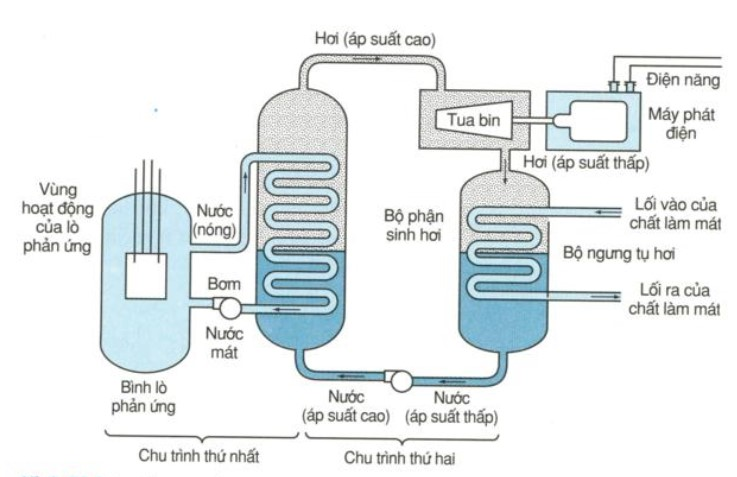
\includegraphics[scale=0.8]{../figs/VN12-PH-49-A-027-1-H1.jpg}
	\end{center}
%	\notebox{
%		Anh chị vẽ lại giùm em hình trên nha.
%	}

\section{Ví dụ minh họa}


\ppgiai{
	Mối liên hệ giữa số mol, khối lượng và số hạt
	\begin{equation}
	n=\dfrac{m}{A}\textrm{ hoặc } n=\dfrac{N}{N_A},
	\end{equation}
	trong đó:
	\begin{itemize}
		\item $m$ là khối lượng chất phóng xạ (tính theo đơn vị g);
		\item $A$ là số khối hay khối lượng mol của chất (tính theo đơn vị g/mol);
		\item $N$ là số nguyên tử có trong khối chất phóng xạ;
		\item $N_A =\SI{6,02e23}{mol^{-1}}$ là số Avôgađrô.
	\end{itemize}
	}

	\viduii{3}{
	[THPT QG - Mã đề 201] Cho rằng một hạt nhân urani $^{235}_{\ 92}\text{U}$ khi phân hạch thì tỏa ra năng lượng là $\SI{200}{\mega\electronvolt}$. Lấy $N_A =\SI{6,02e23}{mol^{-1}}$, và khối lượng mol của urani $^{235}_{\ 92}\text{U}$ là $\SI{235}{\gram/mol}$. Năng lượng tỏa ra khi phân hạch hết $\SI{1}{\kilogram}$ $^{235}_{\ 92}\text{U}$ là
		\begin{mcq}(2)
			\item $\SI{5,12e26}{\mega\electronvolt}$.
			\item $\SI{51,2e26}{\mega\electronvolt}$.
			\item $\SI{2,56e15}{\mega\electronvolt}$.
			\item $\SI{2,56e16}{\mega\electronvolt}$.
		\end{mcq}}{
		\begin{center}
			\textbf{Hướng dẫn giải}
		\end{center}
	
		Số hạt nhân Urani trong $\SI{1}{\kilogram}$ là
		\begin{equation*}
		N=\frac{m}{\mu }{{N}_{A}}=\frac{\SI{1000}{\gram}}{\SI{235}{\gram/mol}}\cdot \SI{6,02e23}{mol^{-1}}=2,5617\cdot 10^{24}.
		\end{equation*}
		
		Năng lượng tỏa ra khi phân hạch hết $\SI{1}{\kilogram}$ $^{235}_{\ 92}\text{U}$ là
		\begin{equation*}
		Q=N\cdot \Delta E = 2,5617\cdot 10^{24} \cdot \SI{200}{\mega\electronvolt}=\SI{5,12e26}{\mega\electronvolt}.
		\end{equation*}
	
		\begin{center}
			\textbf{Câu hỏi tương tự}
		\end{center}	
		
		Trong phản ứng phân hạch U235, năng lượng trung bình tỏa ra khi phân chia một hạt nhân là $ \SI{214}{MeV} $. Tính năng lượng tỏa ra trong quá trình phân hạch $ \SI{1}{g} $ hạt nhân U235 trong lò phản ứng. Cho biết số $ N_{A} = \num{6,023 e23} $, $ \SI{1}{MeV} = \SI{1,6 e-13}{J} $.
		\begin{mcq}(4)
		\item $ \SI{8,8 e4}{J} $.
		\item $ \SI{8,7 e10}{J} $.
		\item $ \SI{8,8 e10}{J} $.
		\item $ \SI{5,5 e10}{J} $.
		\end{mcq}
	
		\textbf{Đáp án:} C.
}
	\viduii{3}{
	[Đề thi đại học khối A, A1 năm 2013]  Một lò phản ứng phân hạch có công suất $\SI{200}{\mega\watt}$. Cho rằng toàn bộ năng lượng mà lò phản ứng này sinh ra đều do sự phân hạch của $^{235}\text{U}$ và đồng vị này chỉ bị tiêu hao bởi quá trình phân hạch. Coi mỗi năm có 365 ngày; mỗi phân hạch sinh ra $\SI{200}{\mega\electronvolt}$; số A-vô-ga-đrô $N_A =\SI{6,02e23}{mol^{-1}}$. Năng lượng mà lò phản ứng tạo ra trong 3 năm là
	\begin{mcq}(4)
		\item $\SI{461,6}{\gram}$.
		\item $\SI{461,6}{\kilogram}$.
		\item $\SI{230,8}{\kilogram}$.
		\item $\SI{230,8}{\gram}$.
	\end{mcq}}{
		\begin{center}
			\textbf{Hướng dẫn giải}
		\end{center}

		Năng lượng mà lò phản ứng tạo ra trong 3 năm là
			\begin{equation*}
			Q=(3\cdot 365\cdot\ 86400)\,\text{s}\cdot \SI{200e6}{\watt}=\SI{1,89216e16}{\joule}.
			\end{equation*}
			
		Vì một phân hạch tạo ra $\SI{200}{\mega\electronvolt}=\SI{3,2e-11}{\joule}$ nên số phân hạch trong 3 năm là 
		\begin{equation*}
		N=\frac{Q}{\SI{3,2e-11}{\joule}}=\frac{\SI{1,89216e16}{\joule}}{\SI{3,2e-11}{\joule}}={5,913\cdot10}^{26}.
		\end{equation*}
		
		Một phân hạch sẽ tiêu hao 1 nguyên tử $^{235}\text{U}$, nên số nguyên tử $^{235}\text{U}$ bị tiêu hao cũng chính là $N={5,913\cdot10}^{26}$
		Số mol $^{235}\text{U}$ bị tiêu thụ là
		\begin{equation*}
		n=\frac{N}{N_A}=\frac{{5,913\cdot10}^{26}}{\SI{6,02e23}{mol^{-1}}}=\SI{982,226}{mol}.
		\end{equation*}
		
		Khối lượng $^{235}\text{U}$ mà lò phản ứng tiêu thụ là
		\begin{equation*}
		m=nA=\SI{982,226}{mol}\cdot\SI{235}{\gram/mol}= \SI{230823,09}{\gram} = \SI{230,8}{\kilogram}.
		\end{equation*}
		
		\begin{center}
			\textbf{Câu hỏi tương tự}
		\end{center}
		
		Giả sử, một nhà máy điện hạt nhân dùng nhiên liệu urani U235. Biết công suất phát điện là $ \SI{500}{MW} $ và hiệu suất chuyển hóa năng lượng hạt nhân thành điện năng là $ 20 \% $. Cho rằng khi một hạt nhân urani U235 phân hạch thì tỏa ra năng lượng là $ \SI{3,2 e-11}{J} $. Lấy $ N_{A} = \SI{6,02 e23}{mol^{-1}} $ và khối lượng mol của U235 là $ \SI{235}{g/mol} $. Nếu nhà máy hoạt động liên tục thì lượng urani U235 mà nhà máy cần dùng trong 365 ngày là
		\begin{mcq}(4)
			\item $ \SI{962}{kg} $.
			\item $ \SI{1121}{kg} $.
			\item $ \SI{1352,5}{kg} $.
			\item $ \SI{1421}{kg} $.
		\end{mcq}	
	
	\textbf{Đáp án:} A.
}




